\documentclass[pdf]{beamer}
\mode<presentation>{} 

\usepackage{hyperref}
\usepackage{pgf}
\usepackage{fancyhdr}
\usepackage{eso-pic}
\usepackage{tikz}
\usetikzlibrary{trees}
\usetikzlibrary{arrows,automata}
\usetikzlibrary{automata,positioning}
\usetikzlibrary{shapes}
\usepackage{tikz-qtree,tikz-qtree-compat}
\usepackage{mathtools,enumerate,amssymb}
\usepackage[utf8]{inputenc}
\usepackage[T1]{fontenc}
\usepackage{graphicx}
\usepackage{multicol}
\usepackage{multirow}
\usepackage{textcomp}
\usepackage[export]{adjustbox}
\usepackage[super]{nth}



\definecolor{Blue}{RGB}{0,0,100}
\definecolor{myBlue}{RGB}{0,0,100}
\definecolor{background}{RGB}{255,255,255}



\title{User Centered Design and Prototyping}
\subtitle{Human Computer Interaction}
\AtBeginSection[]{}



\setbeamertemplate{sidebar right}{}
\setbeamertemplate{footline}{%
\hfill\usebeamertemplate***{navigation symbols}
\hspace{1cm}\insertframenumber{}/\inserttotalframenumber}

\graphicspath{{./img/}}



\begin{document}



{\setbeamercolor{background canvas}{bg=background}
\begin{frame}
\vspace{10mm}
\huge{\raggedleft{\color{black}{\textbf{User Centered Design and Prototyping}}}}

\large{\raggedleft{\color{black} Human Computer Interaction}}

\begin{flushright}
\end{flushright}

\fontsize{7pt}{1pt}\selectfont{
Based on slide deck 

\textbf{Part 3: Designing with the user. User Centered Design and Prototyping}

Human Computer Interaction I: Principles and Design

by

\textbf{Saul Greenberg}
\newline
Professor
\newline
\textbf{University of Calgary, Canada}

\textit{The new slides are marked with a *}
}

\fontsize{5pt}{1pt}\selectfont{ \textcolor{lightgray}
{Slide deck by Saul Greenberg. Permission is granted to use this for non-commercial purposes as long as general credit to Saul Greenberg is clearly maintained.
Warning: some material in this deck is used from other sources without permission. Credit to the original source is given if it is known.}}

\end{frame}}



% Inaintea codului fiecarui slide se vor scrie urmatoarele informatii:
% Nume si prenume student
% Numarul slide-ului corespunzator din prezentarea prof. Saul Greenberg
% Numele imaginilor inserate trebuie sa fie numar_slide_nume_imagine.extensie_imagine



% Morosanu Emil Marian
% slide 1
\begin{frame}
\begin{center}
    \textbf{\LARGE User Centered Design and Prototyping \LARGE}
\end{center}

\bigskip
\bigskip
\bigskip

Why user-centered design is important

Prototyping and user centered design

Prototyping methods

\begin{itemize}
\item
Sketches
\item
Storyboarding
\item
Tutorials as storyboarding
\item
Pictive
\item
Medium fidelity prototypes
\item
Scripted simulations
\item
High fidelity prototypes
\item
Working prototypes
\item
Implementation
\end{itemize}
\end{frame}



% Morosanu Emil Marian
% slide 2
% moro1.PNG 
\begin{frame}
\vspace{8mm}
\textcolor{myBlue}{\textbf{\Large{*System Centered Design}}}

\textcolor{red}{\rule{10cm}{1mm}}

\begin{figure}[b]
    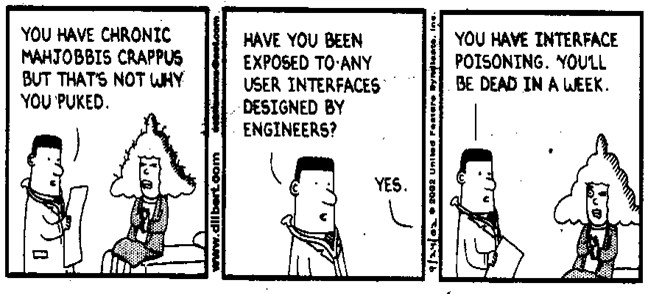
\includegraphics[scale = 0.6]{img2.jpg}
\end{figure}

\url{https://slideplayer.com/slide/7894207/}
\end{frame}



% Morosanu Emil Marian
% slide 3
% moro2.PNG
\begin{frame}
\vspace{8mm}
\textcolor{myBlue}{\textbf{\Large{System Centered Design}}}

\textcolor{red}{\rule{10cm}{1mm}}

\Large{What can I easily build on this platform?}
\bigskip
 
\Large{What can I create from the available tools?}
\bigskip

\Large{What do I as a programmer find interesting?}

\begin{figure}[b]
    	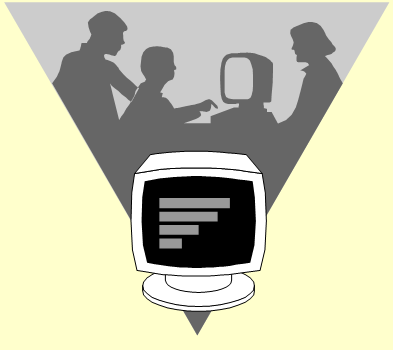
\includegraphics[scale = 0.45]{moro2.PNG}
\end{figure}
\end{frame}



\begin{frame}
\vspace{8mm}
\textcolor{myBlue}{\textbf{\Large{*System Centered Design}}}

\textcolor{red}{\rule{10cm}{1mm}}

\begin{figure}[b]
    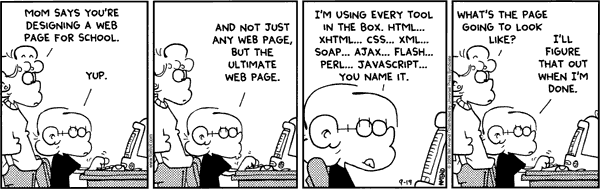
\includegraphics[scale = 0.8]{foxtrot-webdesign.png}
\end{figure}

\url{https://newmedia.report/classes/intro-to-interactives/2016/}
\end{frame}



%Morosanu Emil Marian
% Slide 4
% moro3.PNG
\begin{frame}
\vspace{8mm}
\textcolor{myBlue}{\textbf{\Large{User Centered System Design}}}

\textcolor{red}{\rule{10cm}{1mm}}

Design is based upon a user’s:

\begin{itemize}
    \item[\textcolor{black}{--}] abilities and real needs
    \item[\textcolor{black}{--}] context
    \item[\textcolor{black}{--}] work
    \item[\textcolor{black}{--}] tasks
    \item[\textcolor{black}{--}] need for usable and useful product
    \end{itemize}
    
    \begin{figure}[b]
    	\begin{flushright}
    	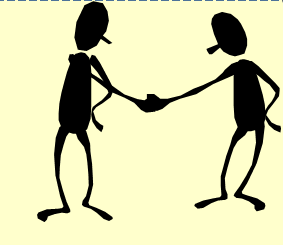
\includegraphics[scale = 0.45]{moro3.PNG}
        \end{flushright}
        
    \end{figure}

	Golden rule of interface design:	\LARGE     \textbf{Know The User}
\end{frame}


%Morosanu Emil Marian
% Slide 5
\begin{frame}
\vspace{8mm}
\textcolor{myBlue}{\textbf{\Large{User Centered System Design}}}

\textcolor{red}{\rule{10cm}{1mm}}

... is based on understanding the domain of work or play in \par which people are engaged and in which they interact with \par computers ...

\bigskip

Assumptions

\begin{itemize}
    \item[\textcolor{black}{--}] The result of a good design is a \textit{satisfied} customer.
    
    \item[\textcolor{black}{--}] The process of design is a \textit{collaboration between designers and  customers }. 

    \item[\textcolor{black}{--}] The design \textit{evolves and adapts to the users} changing concerns, and the process produces a specification as an important byproduct.

    \item[\textcolor{black}{--}] The customer and designer are in \textit{ constant communication } during  the entire process

    \end{itemize}

\begin{flushright}
\textbf{\textit{Denning and Dargan, 1996}}.
\end{flushright}
\end{frame}



%Morosanu Emil Marian
% Slide 6
% moro4.PNG
\begin{frame}
\vspace{8mm}
\textcolor{myBlue}{\textbf{\Large{Participatory Design}}}

\textcolor{red}{\rule{10cm}{1mm}}

{\LARGE Problem \LARGE}

\begin{itemize}
    \item[\textcolor{black}{--}] intuitions wrong
    \item[\textcolor{black}{--}] interviews etc. not precise
    \item[\textcolor{black}{--}] designer cannot know the user sufficiently well to answer all \par issues that come up during the design
\end{itemize}

{\LARGE Solution  \LARGE}
\begin{itemize}
    \item[\textcolor{black}{--}] designers should have access to representative users
    \begin{itemize}
	\item[--] END users, not their managers or union reps!

    \end{itemize}
\end{itemize}

\begin{figure}[b]
    	\begin{flushright}
    	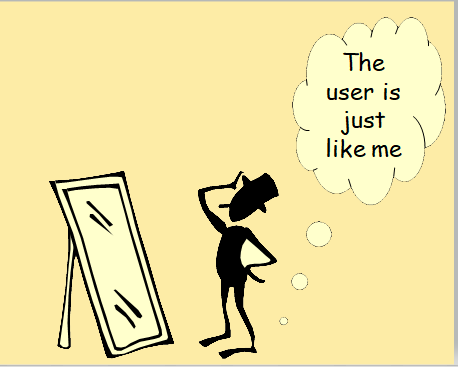
\includegraphics[scale = 0.3]{moro4.PNG}
        \end{flushright}
        \end{figure}
\end{frame}



\begin{frame}
\vspace{8mm}
\textcolor{myBlue}{\textbf{\Large{Participatory Design}}}

\textcolor{red}{\rule{10cm}{1mm}}

\begin{figure}[b]
    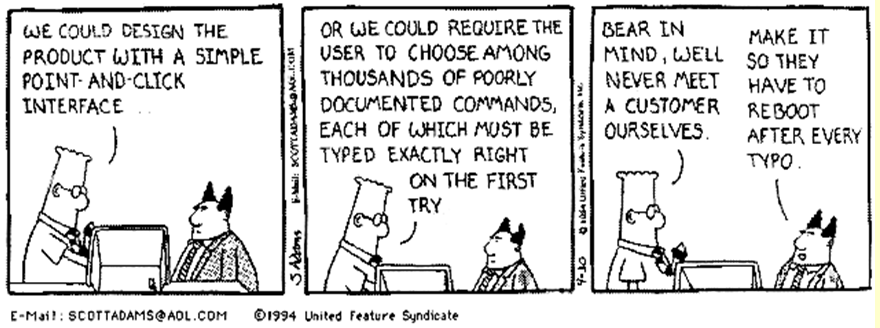
\includegraphics[scale = 0.5]{moro1.PNG}
\end{figure}
\end{frame}



%Morosanu Emil Marian
% Slide 7
% moro5.PNG
\begin{frame}
\vspace{8mm}
\textcolor{myBlue}{\textbf{\Large{Participatory Design}}}

\textcolor{red}{\rule{10cm}{1mm}}

{\LARGE Users are \nth{1} class members in the design process\LARGE}
\begin{itemize}
    \item[\textcolor{black}{--}]active collaborators \textit{vs} passive participants
\end{itemize}

\bigskip

{\LARGE Users considered subject matter experts \LARGE}
\begin{itemize}
    \item[\textcolor{black}{--}]know all about the work context
\end{itemize}

\bigskip

{\LARGE Iterative process \LARGE}
\begin{itemize}
    \item[\textcolor{black}{--}]all design stages subject to revision
\end{itemize}

\begin{figure}[b]
    	\begin{flushright}
    	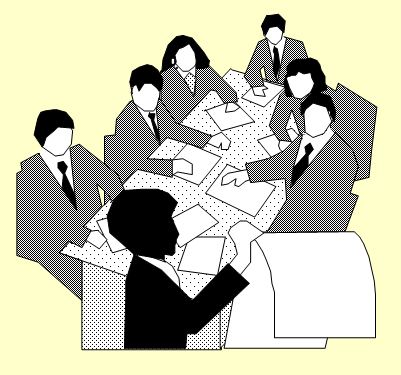
\includegraphics[scale = 0.3]{moro5.PNG}
        \end{flushright}
        \end{figure}
\end{frame}



%/////////////////////////////////////////////////
\begin{frame}
\vspace{8mm}
\textcolor{myBlue}{\textbf{\Large{Participatory Design}}}

\textcolor{red}{\rule{10cm}{1mm}}

\bigskip

{\LARGE Up side \LARGE}

\begin{itemize}
\item users are excellent at reacting to suggested system designs
\begin{itemize}
\item designs must be concrete and visible
\newline
\end{itemize}

\item users bring in important "folk" knowledge of work context
\begin{itemize}
\item knowledge may be otherwise inaccessible to design team
\newline
\end{itemize}

\item
greater buy-in for the system often results
\end{itemize}

\bigskip
\bigskip
\bigskip

\end{frame}



\begin{frame}
\vspace{8mm}
\textcolor{myBlue}{\textbf{\Large{Participatory Design}}}

\textcolor{red}{\rule{10cm}{1mm}}

\bigskip

{\LARGE Down side \LARGE}

\begin{itemize}
\item hard to get a good pool of end users
\begin{itemize}
\item expensive, reluctance ...
\newline
\end{itemize}

\item users are not expert designers
\begin{itemize}
\item do not expect them to come up with design ideas from scratch
\newline
\end{itemize}

\item
the user is not always right
\begin{itemize}
\item do not expect them to  know what they want
\end{itemize}

\end{itemize}

\bigskip
\bigskip
\bigskip

\end{frame}



\begin{frame}
\vspace{8mm}
\textcolor{myBlue}{\textbf{\Large{Methods for involving the user}}}

\textcolor{red}{\rule{10cm}{1mm}}

\bigskip

{\LARGE At the very least, talk to users \LARGE}

\begin{itemize}
    \item[\textcolor{black}{--}] surprising how many designers don’t!
\end{itemize}

\bigskip

{\LARGE Contextual interviews + site visits \LARGE}
\begin{itemize}
    \item[\textcolor{black}{--}] interview users in their workplace, as they are doing their job
    \item[\textcolor{black}{--}] discover user's culture, requirements, expectations, etc.

\end{itemize}

\begin{figure}[b]
    	\begin{flushright}
    	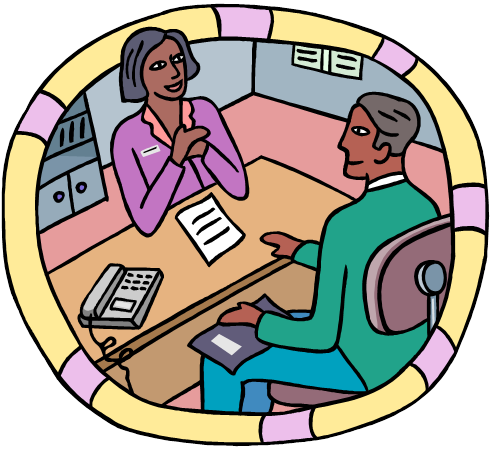
\includegraphics[scale = 0.5]{9.PNG}
        \end{flushright}
        \end{figure}
\end{frame}



\begin{frame}
\vspace{8mm}
\textcolor{myBlue}{\textbf{\Large{Methods for involving the user}}}

\textcolor{red}{\rule{10cm}{1mm}}

\bigskip

{\LARGE Explain designs \LARGE}

\begin{itemize}
    \item[\textcolor{black}{--}] describe what you’re going to do
    \item[\textcolor{black}{--}] get input at all design stages
    \item[\textcolor{black}{--}] all designs subject to revision
\end{itemize}

\bigskip

{\LARGE Important to have visuals and/or demos \LARGE}

\begin{itemize}
    \item[\textcolor{black}{--}] people react far differently with verbal explanations
    \item[\textcolor{black}{--}] this is why prototypes are critical

\end{itemize}

\begin{figure}[b]
    	\begin{flushright}
    	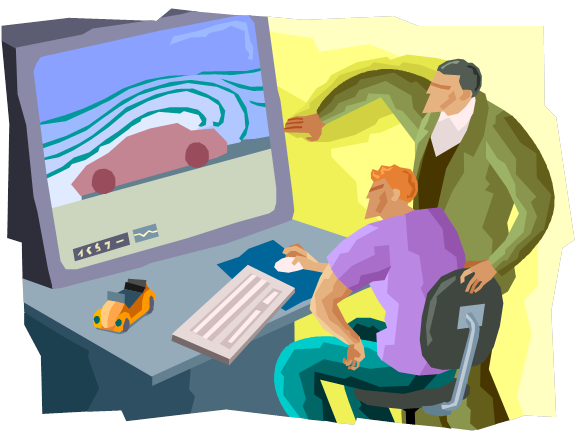
\includegraphics[scale = 0.4]{10.PNG}
        \end{flushright}
        \end{figure}
\end{frame}



\begin{frame}
\vspace{8mm}
\textcolor{myBlue}{\textbf{\Large{Sketching and Prototyping}}}

\textcolor{red}{\rule{10cm}{1mm}}

\bigskip

{\LARGE Sketches/low/medium/high fidelity prototypes \LARGE}

\begin{itemize}
    \item[\textcolor{black}{--}] as investment in design increases, so does the formality of the criteria whereby concepts are reviewed or accepted
\end{itemize}

\begin{figure}[b]
    	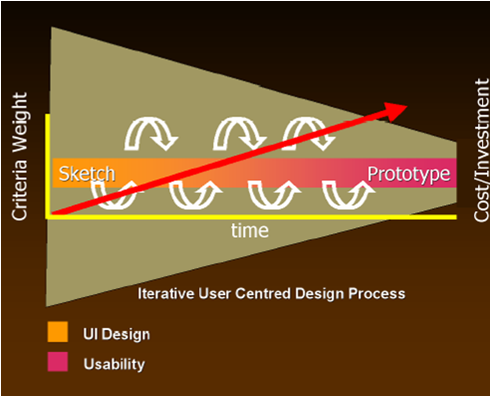
\includegraphics[scale = 0.5]{11.PNG}
\end{figure}
\end{frame}



\begin{frame}
\vspace{8mm}
\textcolor{myBlue}{\textbf{\Large{Sketching and Prototyping}}}

\textcolor{red}{\rule{10cm}{1mm}}

\bigskip

{\LARGE From design to evaluation \LARGE}

\begin{itemize}
    \item[\textcolor{black}{--}] similarly, interface design (idea generation) progresses to usability testing (idea debugging and refinement)

\begin{figure}[b]
    	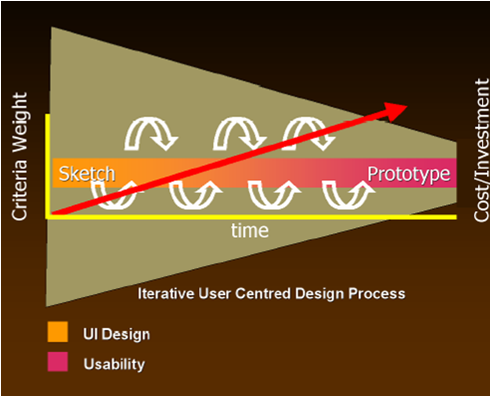
\includegraphics[scale = 0.5]{11.PNG}
\end{figure}
\end{itemize}
\end{frame}



\begin{frame}
\vspace{8mm}
\textcolor{myBlue}{\textbf{\Large{Sketching vs Prototyping}}}

\textcolor{red}{\rule{10cm}{1mm}}

\bigskip

\begin{minipage}[t]{0.4\textwidth}
\begin{itemize}
\item \textbf{Sketches}
\begin{itemize}
\item Invite
\item Suggest
\item Explore
\item Question
\item Propose
\item Provoke
\end{itemize}
\end{itemize}
\end{minipage}
\begin{minipage}[t]{0.4\textwidth}
\begin{itemize}
\item \textbf{Prototypes}
\begin{itemize}
\item Attend
\item Describe
\item Refine
\item Answer
\item Test
\item Resolve
\end{itemize}
\end{itemize}
\end{minipage}

\end{frame}



\begin{frame}
\vspace{8mm}
\textcolor{myBlue}{\textbf{\Large{Sketching vs Prototyping}}}

\textcolor{red}{\rule{10cm}{1mm}}

\begin{center}
\textbf{Early design}
\end{center}

\begin{scriptsize}

\begin{minipage}[b]{0.49\textwidth}
\begin{itemize}
\item Brainstorm different representations
\item Choose a representation
\item Rough out interface style
\newline
\item Task centered walkthrough and redesign
\newline
\item Fine tune interface, screen design
\item Heuristic evaluation and redesign
\item Usability testing and redesign
\newline
\item Limited field testing
\newline
\item Alpha/Beta tests
\end{itemize}
\end{minipage}
\begin{minipage}[b]{0.49\textwidth}
\begin{itemize}
\item Sketches \& low fidelity paper prototypes
\newline
\newline
\newline
\newline
\item Medium fidelity prototypes
\newline
\newline
\newline
\newline
\item High fidelity prototypes
\newline
\item Working systems
\end{itemize}
\end{minipage}

\end{scriptsize}

\begin{center}
\textbf{Late design}
\end{center}

\end{frame}



\begin{frame}
\vspace{8mm}
\textcolor{myBlue}{\textbf{\Large{Sketches \& Low Fidelity Prototypes}}}

\textcolor{red}{\rule{10cm}{1mm}}

\bigskip

{\LARGE \textbf{Paper} mock-up of the interface look, feel, functionality \LARGE}

\begin{itemize}
    \item[\textcolor{black}{--}] quick and cheap to prepare and modify
\end{itemize}

\bigskip

{\LARGE Purpose \LARGE}

\begin{itemize}
    \item[\textcolor{black}{--}] brainstorm competing representations
    \item[\textcolor{black}{--}] elicit user reactions
    \item[\textcolor{black}{--}] elicit user modifications / suggestions

\end{itemize}

\begin{figure}[b]
    	\begin{flushright}
    	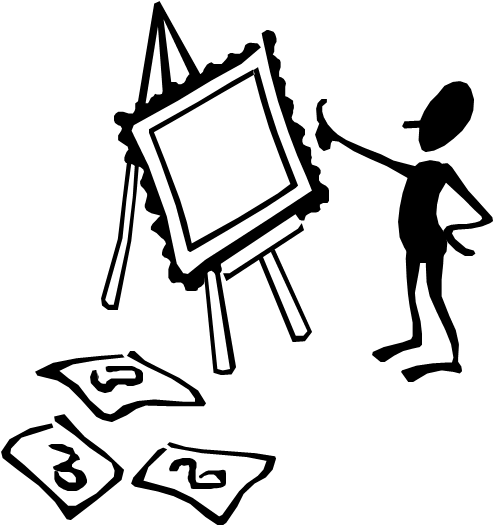
\includegraphics[scale = 0.3]{14.PNG}
        \end{flushright}
        \end{figure}
\end{frame}



\begin{frame}
\vspace{8mm}
\textcolor{myBlue}{\textbf{\Large{*Sketches \& Low Fidelity Prototypes}}}

\textcolor{red}{\rule{10cm}{1mm}}

\begin{figure}[b]
    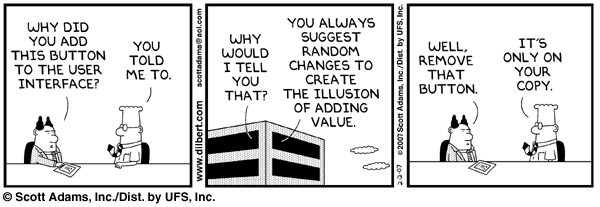
\includegraphics[scale = 0.8]{value_added_illusions.png}
\end{figure}

\url{https://www.cfgigolo.com/2007/02/agregando-valor/index.html}

\end{frame}



\begin{frame}
\vspace{8mm}
\textcolor{myBlue}{\textbf{\Large{Sketches}}}

\textcolor{red}{\rule{10cm}{1mm}}

\bigskip

\begin{itemize}
    \item[\textcolor{black}{--}] drawing of the outward appearance of the intended system
    \item[\textcolor{black}{--}] crudity means people concentrate on high level concepts
    \item[\textcolor{black}{--}] but hard to envision a dialog’s progression

\end{itemize}

\bigskip

\begin{minipage}{0.49\textwidth}
\begin{figure}[b]
   	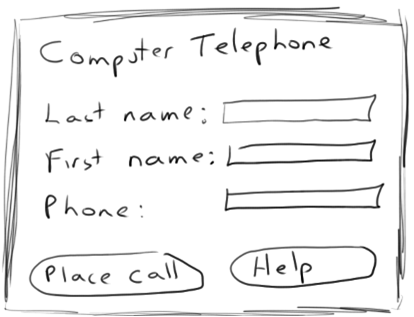
\includegraphics[scale = 0.45]{15a.PNG}
\end{figure}
\end{minipage}
\begin{minipage}{0.49\textwidth}
\begin{figure}[b]
   	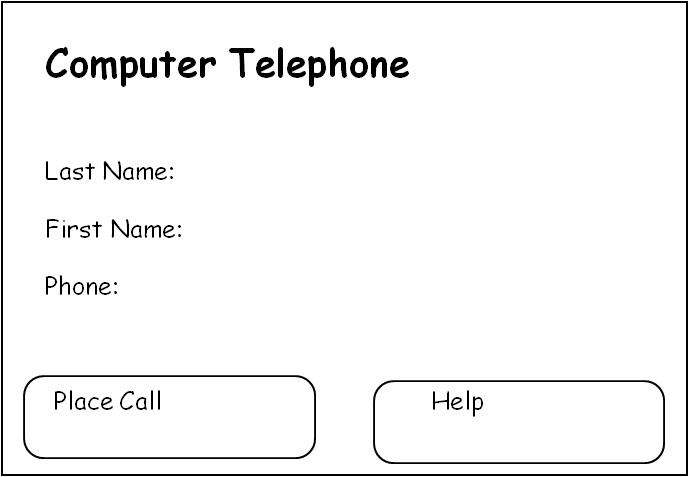
\includegraphics[scale = 0.45]{15b.PNG}
\end{figure}
\end{minipage}

\end{frame}



%/////////////////////////////////////////////////



% Pop Alexandru
% slide 16
%slide16pic.png
\begin{frame}
\vspace{8mm}
\textcolor{myBlue}{\textbf{\Large{Sketches}}}

\textcolor{red}{\rule{10cm}{1mm}}

    \begin{figure}[b]
    	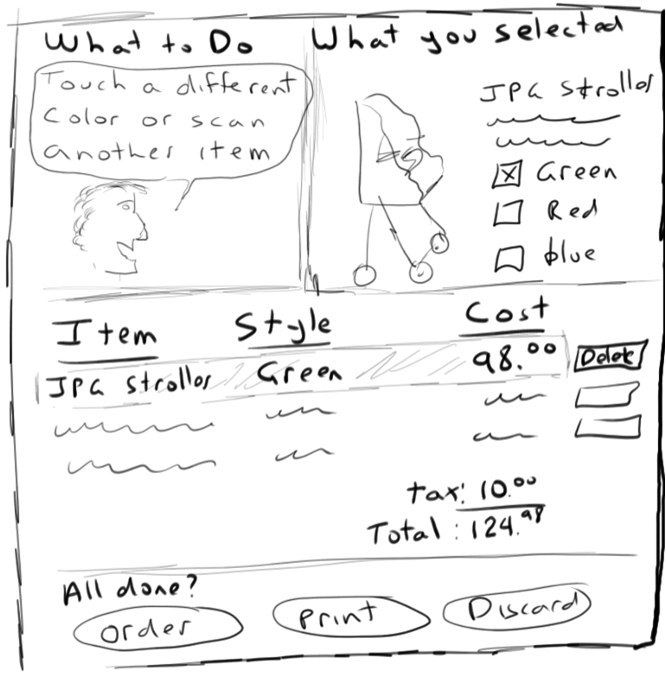
\includegraphics[scale = 0.4]{slide16pic.png}
    \end{figure}
\end{frame}



% Pop Alexandru
% slide 17
%slide17pic.png
\begin{frame}
\vspace{8mm}
\textcolor{myBlue}{\textbf{\Large{Sketches}}}

\textcolor{red}{\rule{10cm}{1mm}}

    \begin{figure}[b]
    	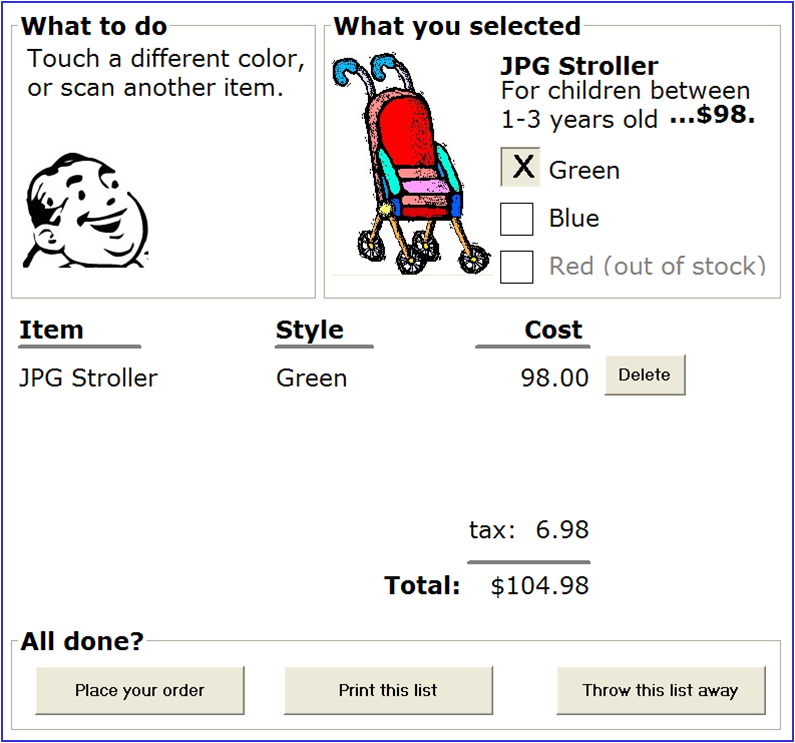
\includegraphics[scale = 0.4]{slide17pic.png}
    \end{figure}
\end{frame}



% Pop Alexandru
% slide 18
\newlength{\seplinewidth}
\newlength{\seplinesep}
\setlength{\seplinewidth}{1mm}
\setlength{\seplinesep}{2mm}
\colorlet{sepline}{red}
\newcommand*{\sepline}{%
  \par
  %\vspace{\dimexpr\seplinesep+.5\parskip}%
  \cleaders\vbox{%
    \begingroup % because of color
      \color{sepline}%
      \hrule width\linewidth height\seplinewidth
    \endgroup
  }\vskip\seplinewidth
  \vspace{-0.85cm}
  %\vspace{\dimexpr\seplinesep-.5\parskip}%
}
\begin{frame}
\vspace{8mm}
\textcolor{myBlue}{\textbf{\Large{The attributes of sketches}}}

\textcolor{red}{\rule{10cm}{1mm}}

\begin{samepage}    
    \begin{multicols}{2}
	\textbf{Quick} \par
    \begin{itemize}
      \item[\textcolor{black}{--}] to make
    \end{itemize}
    \textbf{Timely} \par
    \begin{itemize}
      \item[\textcolor{black}{--}] provided when needed
    \end{itemize}
      \textbf{Disposable} \par
    \begin{itemize}
      \item[\textcolor{black}{--}] investment in the concept, not the execution
    \end{itemize}
      \textbf{Plentiful} \par
    \begin{itemize}
      \item[\textcolor{black}{--}] they make sense in a collection or series of ideas
    \end{itemize}    
	\end{multicols}
   \end{samepage}
\end{frame}



\begin{frame}
\vspace{8mm}
\textcolor{myBlue}{\textbf{\Large{The attributes of sketches}}}

\textcolor{red}{\rule{10cm}{1mm}}

\begin{samepage}    
    \begin{multicols}{2}
      \textbf{Clear vocabulary} \par
    \begin{itemize}
      \item[\textcolor{black}{--}] rendering and style indicates it’s a sketch, not an implementation 
    \end{itemize}
      \textbf{Constrained resolution} \par
    \begin{itemize}
      \item[\textcolor{black}{--}] doesn’t inhibit concept exploration
    \end{itemize}
      \textbf{Consistency with state} \par
    \begin{itemize}
      \item[\textcolor{black}{--}] refinement of rendering matches the actual state of development of the concept 
    \end{itemize}
     \textbf{Suggest and explore rather than confirm} \par
    \begin{itemize}
      \item[\textcolor{black}{--}] value lies in suggesting and provoking what could be i.e., they are the catalyst to conversation and interaction
    \end{itemize}
    
	\end{multicols}
   \end{samepage}
\end{frame}



% Pop Alexandru
% slide 19
% slide19pic.jpg
\begin{frame}
\vspace{8mm}
\textcolor{myBlue}{\textbf{\Large{Storyboarding}}}

\textcolor{red}{\rule{10cm}{1mm}}

\begin{itemize}
      \item[\textcolor{black}{--}] a series of key frames as sketches
      \begin{itemize}
        \item[\textcolor{black}{•}] originally from film; used to get the idea of a scene
        \item[\textcolor{black}{•}] snapshots of the interface at particular points in the interaction
      \end{itemize}
      \item[\textcolor{black}{--}] users can evaluate quickly the direction the interface is heading
      \newline
      \item \textbf{note how each scene in this storyboard is annotated}
      
      Source: \url{https://www.storyboardthat.com/}
      
  \end{itemize}
\end{frame}



% Pop Alexandru
% slide 20
%slide20pic.png
\begin{frame}
\vspace{8mm}
\textcolor{myBlue}{\textbf{\Large{*Storyboarding}}}

\textcolor{red}{\rule{10cm}{1mm}}

\begin{figure}[b]
  	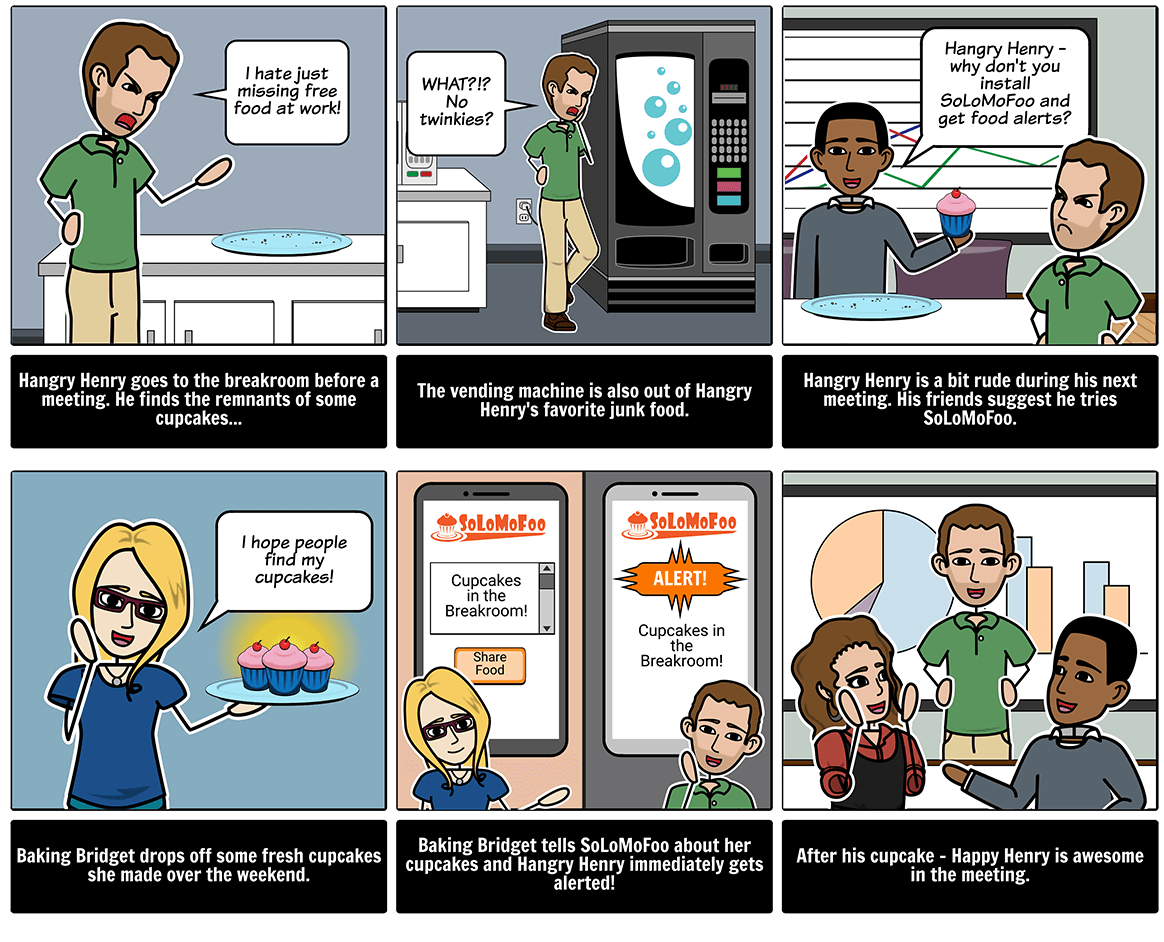
\includegraphics[scale = 0.22]{solomofoo-product-pitch.png}
\end{figure}
    
\end{frame}



% Pop Alexandru
% slide 21
%slide21pic1.png
%slide21pic2.png
%slide21pic3.png
%slide21pic4.png
\begin{frame}
\vspace{8mm}
\textcolor{myBlue}{\textbf{\Large{Storyboarding}}}

\textcolor{red}{\rule{10cm}{1mm}}

\begin{columns}[t]
\column{.12\textwidth}
\vspace{-2cm}
\tiny\centerline {Initial}
\tiny\centerline {screen} \vspace{3cm} \hfill \break
\hfill \linebreak
\tiny\centerline {Change}
\tiny\centerline {the}
\tiny\centerline {color\textrightarrow}
\column{.38\textwidth}
\hspace{-1.3cm}
\centering
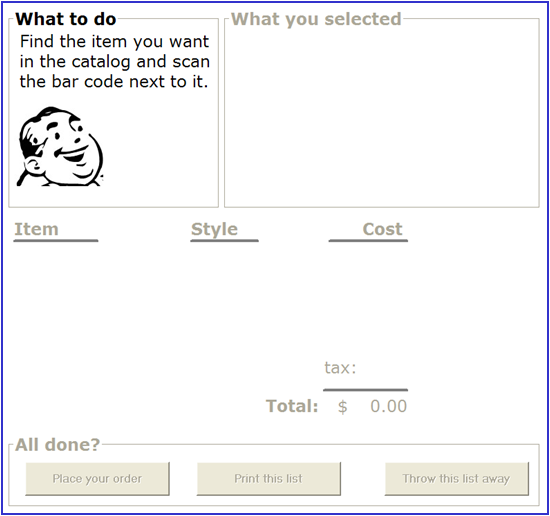
\includegraphics[width=4cm,height=4cm]{slide21pic1.png}\\
\hspace{-1.3cm}
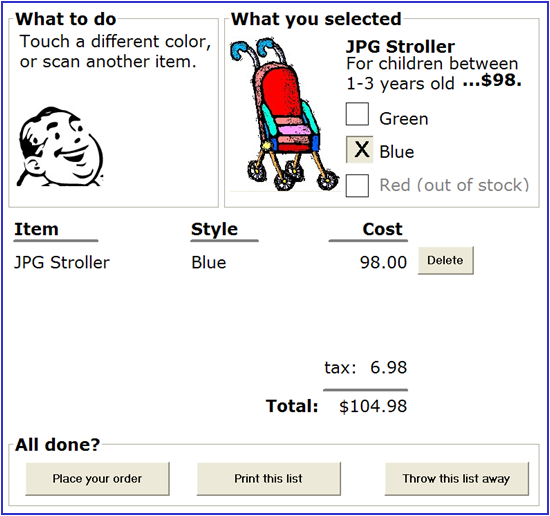
\includegraphics[width=4cm,height=4cm]{slide21pic2.png} 
\column{.12\textwidth}
\vspace{-2cm}
\tiny\centerline {Scan the}
\tiny\centerline {stroller\textrightarrow} \vspace{3cm} \hfill \break
\hfill \linebreak
\tiny\centerline {Place the}
\tiny\centerline {order\textrightarrow}
\column{.38\textwidth}
\centering
\hspace{-1.3cm}
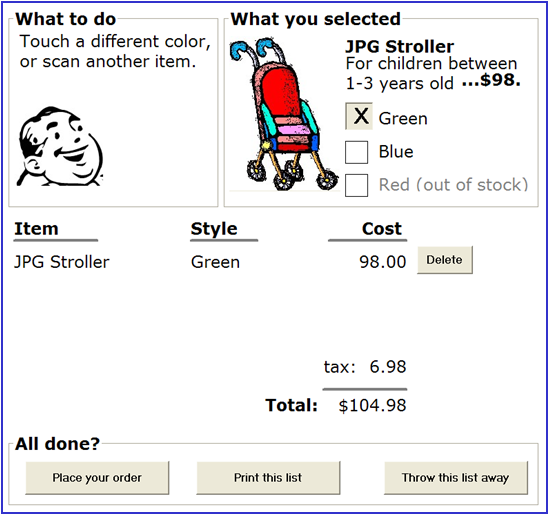
\includegraphics[width=4cm,height=4cm]{slide21pic3.png}\\
\hspace{-1.3cm}
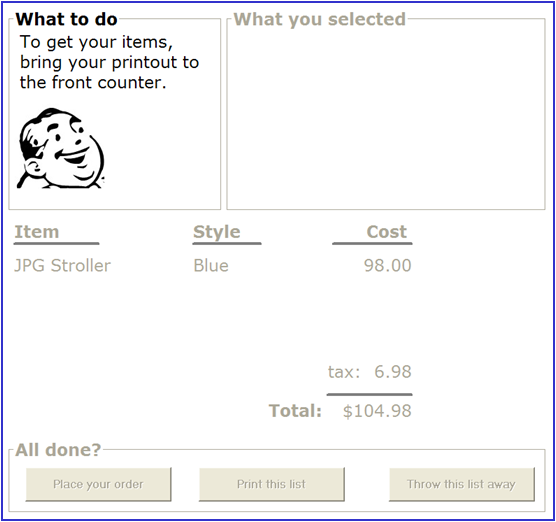
\includegraphics[width=4cm,height=4cm]{slide21pic4.png}
\end{columns}
\end{frame}



% Pop Alexandru
% slide 22
%slide22pic1.png
%slide22pic2.png
%slide22pic3.png
%slide22pic4.png
\begin{frame}
\vspace{8mm}
\textcolor{myBlue}{\textbf{\Large{Storyboarding}}}

\textcolor{red}{\rule{10cm}{1mm}}

\begin{columns}[t]
\column{.12\textwidth}
\vspace{-2cm}
\tiny\centerline {Alternate}
\tiny\centerline {path...} \vspace{3cm} \hfill \break
\hfill \linebreak
\tiny\centerline {Touch}
\tiny\centerline {previous}
\tiny\centerline {item\textrightarrow}
\column{.38\textwidth}
\hspace{-1.3cm}
\centering
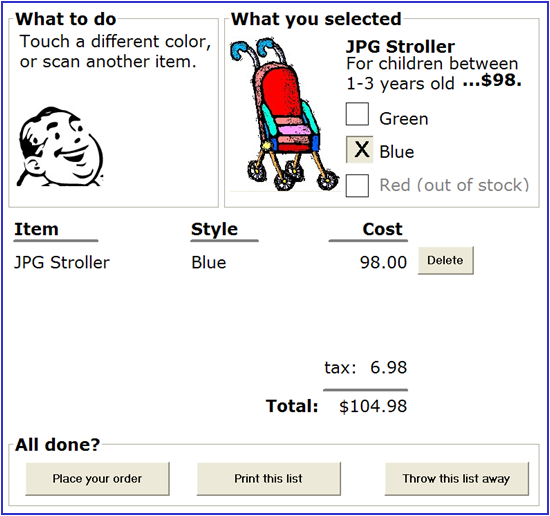
\includegraphics[width=4cm,height=4cm]{slide22pic1.png}\\
\hspace{-1.3cm}
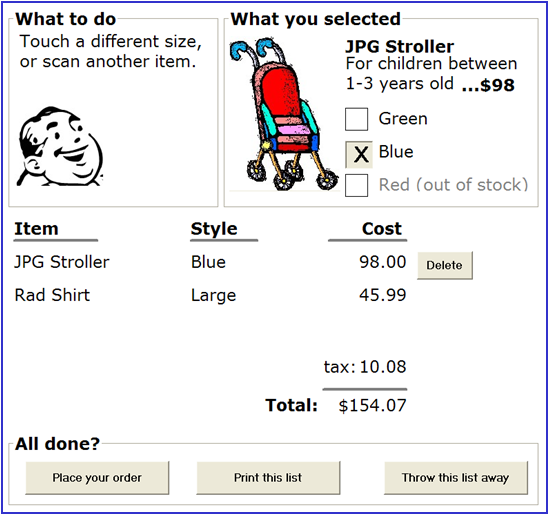
\includegraphics[width=4cm,height=4cm]{slide22pic2.png} 
\column{.12\textwidth}
\vspace{-2cm}
\tiny\centerline {Scan the}
\tiny\centerline {shirt\textrightarrow} \vspace{3cm} \hfill \break
\hfill \linebreak
\tiny\centerline {Delete}
\tiny\centerline {that}
\tiny\centerline {item\textrightarrow}
\column{.38\textwidth}
\centering
\hspace{-1.3cm}
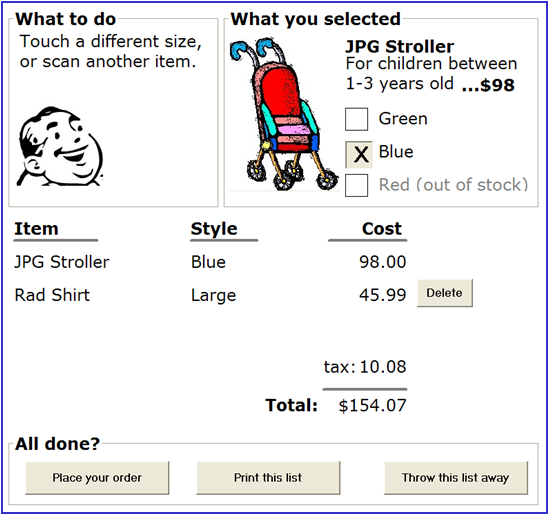
\includegraphics[width=4cm,height=4cm]{slide22pic3.png}\\
\hspace{-1.3cm}
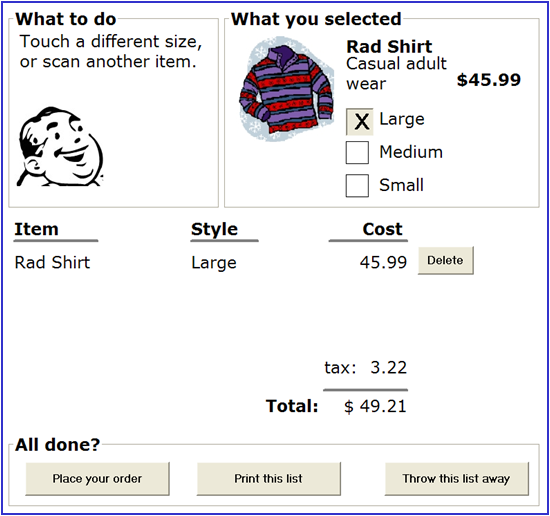
\includegraphics[width=4cm,height=4cm]{slide22pic4.png}
\end{columns}
\end{frame}



%Scurtu Andreea
% slide 42
\begin{frame}
\vspace{8mm}
\textcolor{myBlue}{\textbf{\Large{Storyboard of a computer telephone}}}

\textcolor{red}{\rule{10cm}{1mm}}

\bigskip
\bigskip
\bigskip
\bigskip
 	\begin{picture}(0,0)
		\put(-10,-20){\hbox{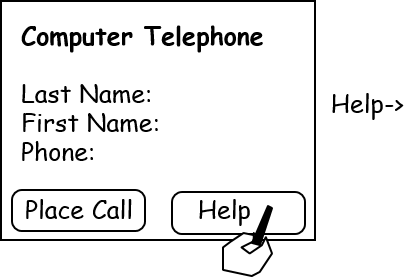
\includegraphics[scale=0.50]{42_1.png}}}
	\end{picture}
    
    \begin{picture}(0,0)
		\put(93,-7){\hbox{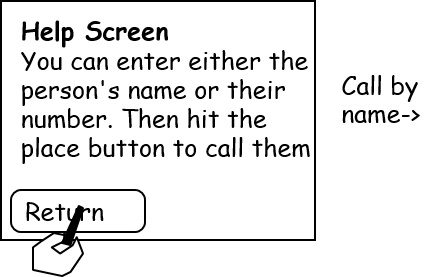
\includegraphics[scale=0.50]{42_2.png}}}
	\end{picture}
    
    \begin{picture}(0,0)
		\put(200,4){\hbox{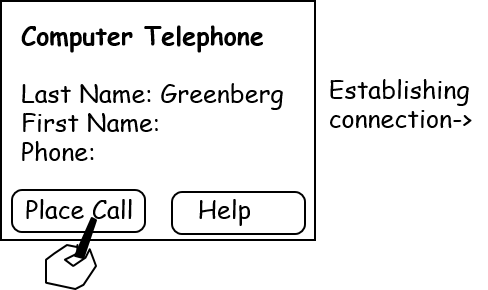
\includegraphics[scale=0.50]{42_3.png}}}
	\end{picture}
    
    \begin{picture}(0,0)
		\put(-10,-80){\hbox{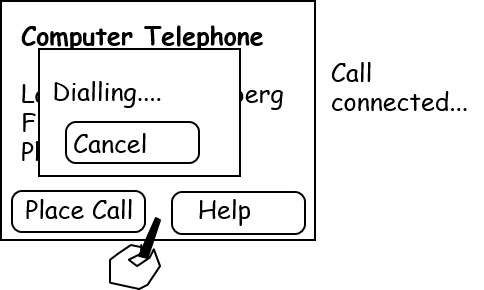
\includegraphics[scale=0.50]{42_4.png}}}
	\end{picture}
    
    \begin{picture}(0,0)
		\put(107,-54){\hbox{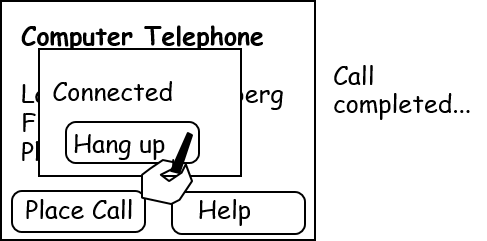
\includegraphics[scale=0.50]{42_5.png}}}
	\end{picture}
    
    \begin{picture}(0,0)
		\put(225,-40){\hbox{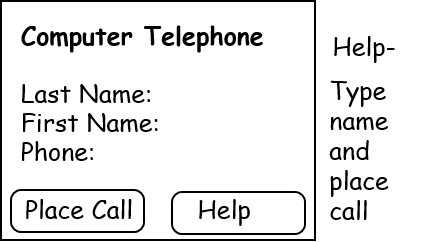
\includegraphics[scale=0.50]{42_6.png}}}
	\end{picture}

\end{frame}



%Popescu Adrian
%slide 24
\begin{frame}
\vspace{8mm}
\textcolor{myBlue}{\textbf{\Large{Tutorials as storyboarding}}}

\textcolor{red}{\rule{10cm}{1mm}}

\begin{itemize}
\item [--]a step by step storyboard walk-through with detailed explanations
\item[--]written in advance of the system implementation
\item[--]also serves as an interface specification for programmers
\end{itemize}

	\begin{figure}[b]
      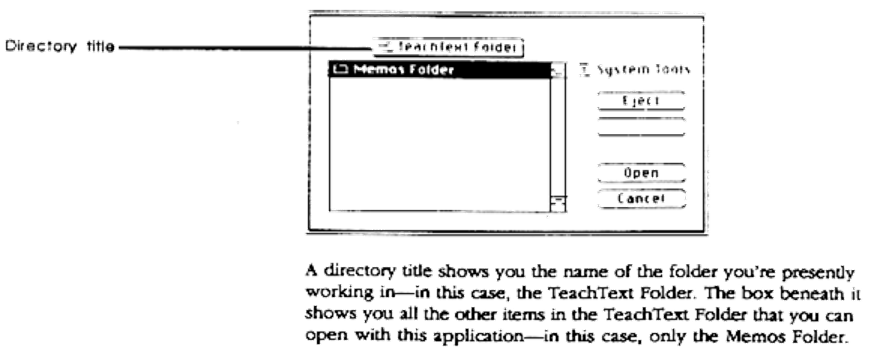
\includegraphics[scale = 0.47, right]{24_Picture1.png}
  	\end{figure}

\raggedright 
\fontsize{2pt}{1pt}\selectfont{\color{gray}Apple’s Tutorial Guide to the Macintosh Finder
}
 
\end{frame}



%Popescu Adrian
%slide 25
\begin{frame}
\vspace{8mm}
\textcolor{myBlue}{\textbf{\Large{ \textbf{Pictive}\tiny{plastic interface for collaborative technology initiatives through video exploration}}}}

\textcolor{red}{\rule{10cm}{1mm}}

\textbf{designing with office supplies}
\begin{itemize}
\item [--] multiple layers of sticky notes and plastic overlays
\item[--]different sized stickies represent icons, menus, windows etc.
\end{itemize}

\textbf{interaction demonstrated by manipulating notes}
\begin{itemize}
\item [--]new interfaces built on the fly
\end{itemize}

\textbf{session videotaped for later analysis}
\begin{itemize}
\item [--]usually end up with mess of paper and plastic!
\end{itemize}

\begin{picture}(0,0)
    \put(250,-45)
	{\hbox{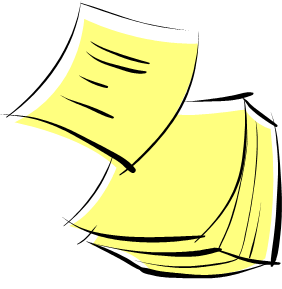
\includegraphics[width=2.5 cm]{25_Picture2.png}}}
\end{picture}

\begin{picture}(0,0)
    \put(200,-45)
	{\hbox{
\includegraphics[width=2.5 cm]{25_Picture1.png}}}
\end{picture}

\end{frame}



%Popescu Adrian
%slide 26
\begin{frame}
\vspace{8mm}
\textcolor{myBlue}{\textbf{\Large{Pictive}}}

\textcolor{red}{\rule{10cm}{1mm}}

\textbf{Can pre-make paper interface components}

\vspace{2px}{button}

\begin{picture}(0,0)
    \put(0,-9)
	{\hbox{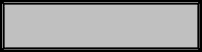
\includegraphics[width=2.5 cm]{26_Picture1.png}}}
\end{picture}

\vspace{0.8cm}{combo box}

\begin{picture}(0,0)
    \put(0,-6)
	{\hbox{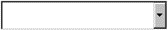
\includegraphics[width=3 cm]{26_Picture2.png}}}
\end{picture}

\vspace{0.8cm}{list box}

\begin{picture}(0,0)
    \put(0,-60)
	{\hbox{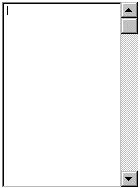
\includegraphics[width=1.8 cm]{26_Picture3.png}}}
\end{picture}

\begin{picture}(0,0)
    \put(250,50)
	{\hbox{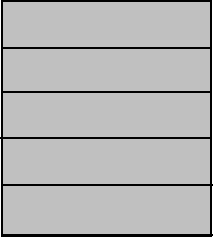
\includegraphics[width=2.5 cm]{26_Picture4.png}}}
\end{picture}

\begin{picture}(0,0)
    \put(250,-10)
	{\hbox{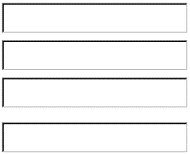
\includegraphics[width=2.5 cm]{26_Picture5.png}}}
\end{picture}

\begin{picture}(0,0)
    \put(120,100)
	{\hbox{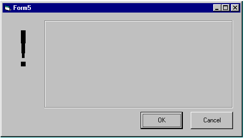
\includegraphics[width=3.5 cm]{26_Picture6.png}}}
\end{picture}

\begin{picture}(0,0)
    \put(120,0)
	{\hbox{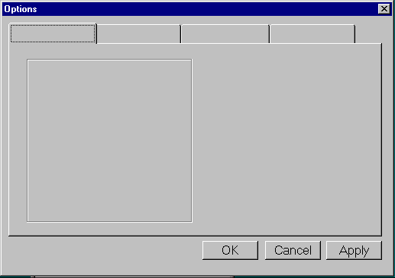
\includegraphics[width=3.5 cm]{26_Picture7.png}}}
\end{picture}
\end{frame}



%Popescu Adrian
%slide 27
\begin{frame}
\vspace{8mm}
\textcolor{myBlue}{\textbf{\Large{Medium fidelity prototypes}}}

\textcolor{red}{\rule{10cm}{1mm}}

\textbf{prototyping with a computer}
\begin{itemize}
\item [--]simulate some but not all features of the interface
\begin{itemize}
\item [$\bullet$]engaging for end users
\end{itemize}
\end{itemize}

\textbf{purpose}
\begin{itemize}
\item[--] provides sophisticated but limited scenario for the user to try
\item[--] can test more subtle design issues
\end{itemize}

\textbf{dangers}
\begin{itemize}
\item [--]user’s reactions often "in the small"
\item[--]users reluctant to challenge designer
\item[--]users reluctant to touch the design
\item[--]management may think its real!

\end{itemize}

\end{frame}



%Popescu Adrian
%slide 30
\begin{frame}
\vspace{8mm}
\textcolor{myBlue}{\textbf{\Large{Medium fidelity prototypes}}}

\textcolor{red}{\rule{10cm}{1mm}}

\textbf{draw each storyboard scene on computer
}
\begin{itemize}
\item [--]very thin horizontal prototype
\item[--] does not capture the interaction "feel"
\end{itemize}

\begin{figure}
	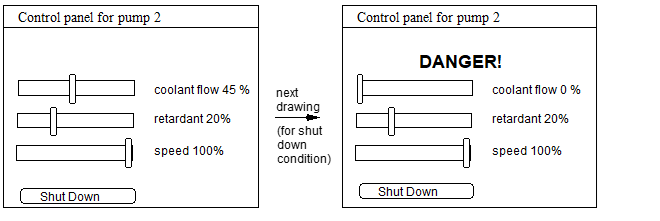
\includegraphics[width=10 cm]{30_Picture1.png}
\end{figure}
\end{frame}



% Ruica Cristina
% slide 31
\begin{frame}
\vspace{8mm}
\textcolor{myBlue}{\textbf{\Large{Scripted simulations}}}

\textcolor{red}{\rule{10cm}{1mm}}

\hfill \linebreak
\textbf{create storyboard with media tools}
\begin{itemize}
      \item[\textcolor{black}{--}] scene transition activated by simple user inputs      
      \item[\textcolor{black}{--}]a simple vertical prototype
  \end{itemize}
  
  \hfill \linebreak
\textbf{user given a very tight script/task to follow}
\begin{itemize}
      \item[\textcolor{black}{--}] appears to behave as a real system
		\item[\textcolor{black}{--}]script deviations blow the simulation     
  \end{itemize}
   
  \begin{tikzpicture}
  \node (img1)  at (1.8,3) {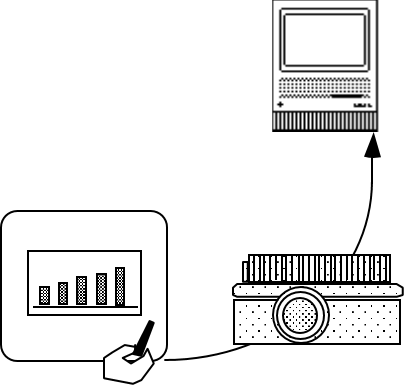
\includegraphics[height=3.5cm, right]{31_1.png}};
  \pause
  \node (img2) at (2,3) {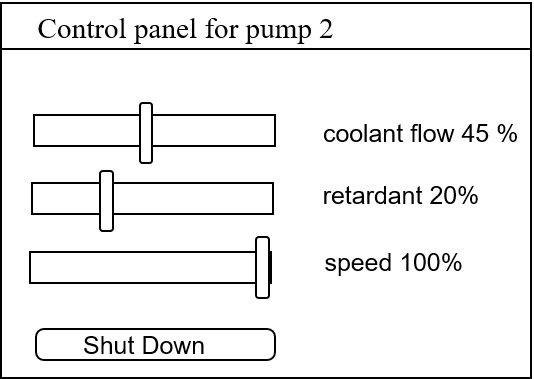
\includegraphics[height=3.5cm, right]{31_2.png}};
  \pause
  \node (img3) at (3,1.3) {
\includegraphics[height=0.5cm]{31_3.png}};
  \pause
  \node (img4) at (2,3) {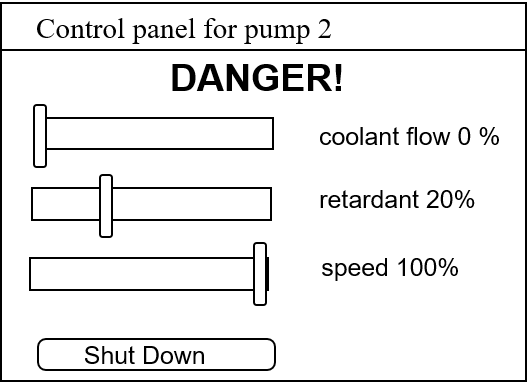
\includegraphics[height=3.6cm, right]{31_4.png}};  
\end{tikzpicture}    
\end{frame}



% Ruica Cristina
% slide 32
\begin{frame}
\vspace{8mm}
\textcolor{myBlue}{\textbf{\Large{Scripted simulations}}}

\textcolor{red}{\rule{10cm}{1mm}}
   
  \begin{tikzpicture}
  \node (img1)  at(-1,0) {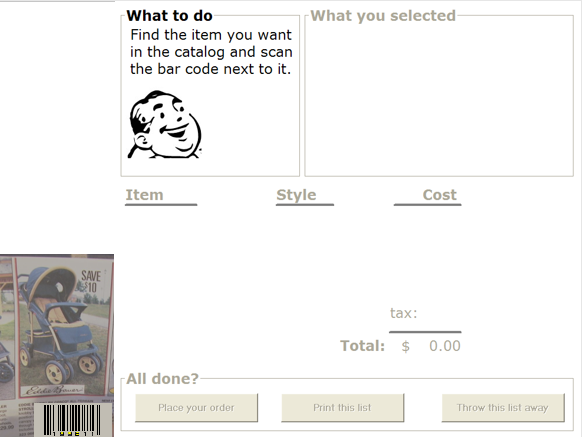
\includegraphics[scale=0.5]{32_1.png}};
  \pause
  \node (img2) at (-1.7,-2) {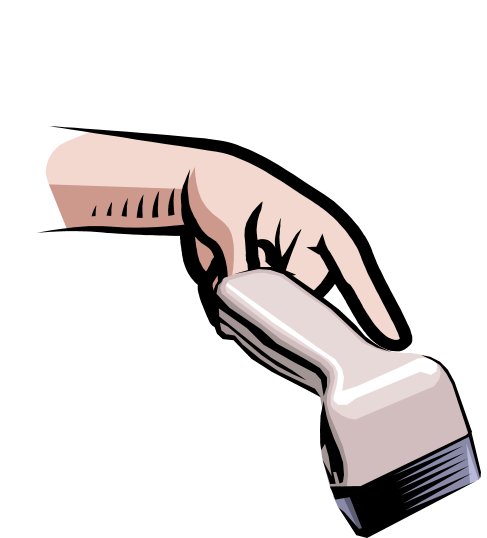
\includegraphics[height=3cm,left]{32_2.png}};  
\end{tikzpicture}    
\end{frame}



% Ruica Cristina
% slide 33
\begin{frame}
\vspace{8mm}
\textcolor{myBlue}{\textbf{\Large{Scripted simulations}}}

\textcolor{red}{\rule{10cm}{1mm}}

\begin{tikzpicture}
  \node (img3)  at (0,0) {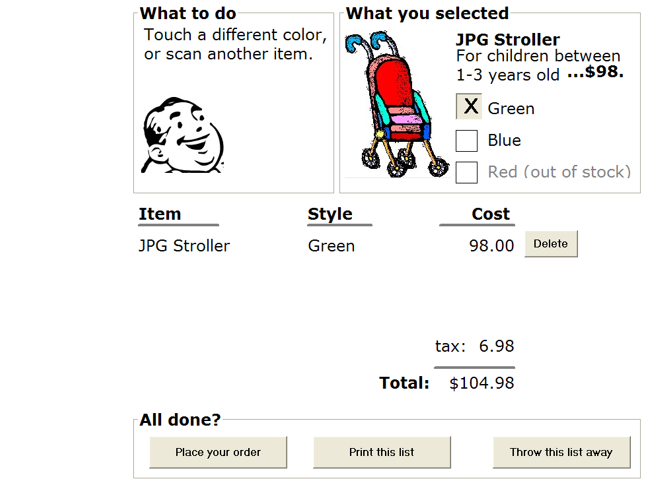
\includegraphics[scale=0.5]{33_1.png}};
  \pause
  \node (img4) at (0,0){\includegraphics[scale=0.5]{33_2.png}};
  \end{tikzpicture} 
 \end{frame}



% Ruica Cristina
% slide 34
\begin{frame}
\vspace{8mm}
\textcolor{myBlue}{\textbf{\Large{Scripted simulations}}}

\textcolor{red}{\rule{10cm}{1mm}}

\begin{tikzpicture}
  \node (img5)  at (0,0) {\includegraphics[scale=0.6]{34_1.png}};
  \pause
  \node (img6) at (0,0.0){\includegraphics[scale=0.6]{34_2.png}};
  
\end{tikzpicture} 
    
\end{frame}



% Ruica Cristina
% slide 35
\begin{frame} 
\vspace{8mm}
\textcolor{myBlue}{\textbf{\Large{Scripted simulations}}}

\textcolor{red}{\rule{10cm}{1mm}}

    \begin{figure}[b]
    	\includegraphics[scale = 0.55]{35_1.png}
    \end{figure}
\end{frame}



\begin{frame}
\vspace{8mm}
\textcolor{myBlue}{\textbf{\Large{*High fidelity prototypes}}}

\textcolor{red}{\rule{10cm}{1mm}}

\textbf{Prototyping tools}
\begin{itemize}
\item \textbf{Axure}

\url{https://www.axure.com/}

\item \textbf{Balsamiq Mockups}

\url{https://balsamiq.com/}

\item \textbf{HotGloo}

\url{https://www.hotgloo.com/}

\item \textbf{MockFlow}

\url{https://www.mockflow.com/}
\newline

\item \url{http://lmgtfy.com/?q=online+prototyping+tools}
\end{itemize}

\end{frame}



\begin{frame}
\vspace{8mm}
\textcolor{myBlue}{\textbf{\Large{*Working prototypes}}}

\textcolor{red}{\rule{10cm}{1mm}}

\begin{itemize}
\item[--] \textbf{simple algorithms }
\begin{itemize}
\item ignore special cases
\end{itemize}

\item[--] \textbf{fake data}
\begin{itemize}
\item similar data, images instead of videos, etc.
\end{itemize}

\item[--] \textbf{Wizard of Oz}
\begin{itemize}
\item human expert operating behind the scenes to simulate interface responses
\end{itemize}

\end{itemize}

\end{frame}



%Popescu Adrian
%slide 28
\begin{frame}
\vspace{8mm}
\textcolor{myBlue}{\textbf{\Large{Working prototypes}}}

\textcolor{red}{\rule{10cm}{1mm}}

\textbf{vertical prototypes}
\begin{itemize}
\item[--] includes in-depth functionality for only a few selected features
\item[--]common design ideas can be tested in depth
\end{itemize}

\textbf{horizontal prototypes}
\begin{itemize}
\item [--]the entire surface interface with no underlying functionality
\item[--]a simulation; no real work can be performed
\end{itemize}

\textbf{scenario prototypes}
\begin{itemize}
\item [--] only features and functionality along the specific scenarios or paths
\end{itemize}

\begin{picture}(0,0)
    \put(113,-45)
	{\hbox{\includegraphics[width=6 cm]{28_Picture1.png}}}
\end{picture}

\vspace{2.4cm} \hspace{-1cm}
\raggedright 
\fontsize{2pt}{1pt}\selectfont{\color{gray}Nielsen, J. (1993) Usability Engineering, p93-101, Academic Press. 
}

\end{frame}



% Ruica Cristina
% slide 36
\begin{frame}
\vspace{8mm}
\textcolor{myBlue}{\textbf{\Large{Implementation}}}

\textcolor{red}{\rule{10cm}{1mm}}

\begin{itemize}
\item design tools for laying out common widgets 
\item excellent for showing look and feel
\begin{itemize}
      \item[\textcolor{black}{--}] a broader horizontal prototype
      
      \item[\textcolor{black}{--}] but constrained to widget library
  \end{itemize}
  
\item vertical functionality added selectively
\begin{itemize}
      \item[\textcolor{black}{--}] through programming
  \end{itemize}
  \begin{figure}[b]
    	\includegraphics[scale = 0.5,right]{36_1.png}
    \end{figure}
\item already covered in introduction
\end{itemize}
\end{frame}



% Ruica Cristina
% slide 37
\begin{frame}
\vspace{8mm}
\textcolor{myBlue}{\textbf{\Large{Wizard of Oz}}}

\textcolor{red}{\rule{10cm}{1mm}}

aka \textbf{Wizard of Oz Experiment}

A method of testing a system that does not exist

\begin{itemize}
      \item[\textcolor{black}{--}] the listening typewriter, IBM 1984      
      
  \end{itemize}
  \begin{figure}[b]
    	\includegraphics[scale = 0.5]{37_1.png}
    \end{figure}
    What the user sees
    
   \AddToShipoutPictureFG*{
    \AtPageLowerLeft{\put(-200,2){\makebox[\paperwidth][r]{\fontsize{4pt}{1pt}\selectfont{\color{gray}{From Gould, Conti \& Hovanvecz, Comm ACM 26(4) 1983.
}}}}}  
    }
    \AddToShipoutPictureFG*{
    \AtPageLowerLeft{\put(-2,2){\makebox[\paperwidth][r]{\fontsize{4pt}{1pt}\selectfont{\color{gray}{Saul Greenberg}}}}}  
    }
\end{frame}



% Scurtu Andreea
% slide 38
\begin{frame}
\vspace{8mm}
\textcolor{myBlue}{\textbf{\Large{Wizard of Oz}}}

\textcolor{red}{\rule{10cm}{1mm}}

aka \textbf{Wizard of Oz Experiment}

A method of testing a system that does not exist

\begin{itemize}
      \item[\textcolor{black}{--}] the listening typewriter, IBM 1984      
      
  \end{itemize}
  \begin{figure}[b]
    	\includegraphics[scale = 0.7]{38_1.png}
  \end{figure}
  
  \leavevmode\makebox(0,0){\put(30,45){ What the user sees }}
  \leavevmode\makebox(0,0){\put(180,45){ The wizard }}
     
  \lfoot{From Gould, Conti  Hovanvecz, Comm ACM 26(4) 1983.}

\end{frame}



%Scurtu Andreea
% slide 39
\begin{frame}
\vspace{8mm}
\textcolor{myBlue}{\textbf{\Large{Wizard of Oz}}}

\textcolor{red}{\rule{10cm}{1mm}}

Human "wizard" simulates system response

\begin{itemize}
      \item[\textcolor{black}{--}] interprets user input according to an algorithm

      \item[\textcolor{black}{--}] controls computer to simulate appropriate output    
        
      \item[\textcolor{black}{--}] uses real or mock interface
      
      \item[\textcolor{black}{--}] wizard sometimes visible, sometimes hidden

 	\begin{itemize}
    	\item[\textcolor{black}{•}] "pay no attention to the man behind the curtain!"
    \end{itemize}

  \end{itemize}
  
  \bigskip
 good for:

	\begin{itemize}
    	\item[\textcolor{black}{--}] adding simulated and complex vertical functionality
      
        \item[\textcolor{black}{--}] testing futuristic idea
          
  \end{itemize}
  
    \begin{picture}(0,0)
		\put(270,-40){\hbox{\includegraphics[scale=0.50]{39_1.png}}}
	\end{picture}
    
\end{frame}



% Scurtu Andreea
% slide 43
\begin{frame}
\vspace{8mm}
\textcolor{myBlue}{\textbf{\Large{Wizard of Oz - Examples}}}

\textcolor{red}{\rule{10cm}{1mm}}

\bigskip
{\Large IBM: an imperfect listening typewriter using continuous speech recognition}

	\begin{itemize}
      \item[\textcolor{black}{--}] secretary trained to:
      \begin{itemize}
        \item[\textcolor{black}{•}] understand key words as "commands"
        \item[\textcolor{black}{•}] to type responses on screen as the system would
        \item[\textcolor{black}{•}] manipulating graphic images through gesture and speech
      \end{itemize}
  \end{itemize}
  
 \bigskip
{\Large Intelligent Agents / Programming by demonstration}

\begin{itemize}
      \item[\textcolor{black}{--}] person trained to mimic "learning agent"
      \begin{itemize}
        \item[\textcolor{black}{•}] user provides examples of task they are trying to do
        \item[\textcolor{black}{•}]computer learns from them
      \end{itemize}
      \item[\textcolor{black}{--}] shows how people specify their tasks
\end{itemize}

 \bigskip
 {\Large In both cases, system very hard to implement, even harder to change!} 
\end{frame}



\begin{frame}
\vspace{8mm}
\textcolor{myBlue}{\textbf{\Large{*Wizard of Oz - Examples}}}

\textcolor{red}{\rule{10cm}{1mm}}

\bigskip
{\Large \textbf{Facebook}}

\begin{itemize}
\item \textit{Facebook M}, the social network’s text-based virtual assistant
\item it was shut down on 19th of January 2018
\newline
\end{itemize}

\url{https://www.theverge.com/2015/10/26/9605526/facebook-m-hands-on-personal-assistant-ai}
\newline

\url{https://medium.com/@Ganticdotco/the-ibm-test-is-a-great-example-of-a-wizard-of-oz-experiment-edbf62d65349}
\end{frame}



%Popescu Adrian
%slide 29
\begin{frame}
\vspace{8mm}
\textcolor{myBlue}{\textbf{\Large{Integrating prototypes and products}}}

\textcolor{red}{\rule{10cm}{1mm}}

\textbf{throw-away}
\begin{itemize}
\item [--]prototype only serves to elicit user reaction
\item[--]creating prototype must be rapid, otherwise too expensive
\end{itemize}

\textbf{incremental}
\begin{itemize}
\item [--]product built as separate components (modules)
\item[--]each component prototyped \& tested, then added to the final system
\end{itemize}

\textbf{evolutionary}
\begin{itemize}
\item [--]prototype altered to incorporate design changes
\item[--]eventually becomes the final product
\end{itemize}

\end{frame}



\begin{frame}
\vspace{8mm}
\textcolor{myBlue}{\textbf{\Large{*Integrating prototypes and products}}}

\textcolor{red}{\rule{10cm}{1mm}}

\begin{itemize}
\item
historically - discard the prototype away and implement the final design from scratch
\newline

\item agile development and designing in the web browser produces change
\begin{itemize}
\item incrementally and evolutionary develop a prototype until it becomes the product
\end{itemize}
\end{itemize}

\end{frame}



%Scurtu Andreea
% slide 40
\begin{frame}
\vspace{8mm}
\textcolor{myBlue}{\textbf{\Large{What you now know}}}

\textcolor{red}{\rule{10cm}{1mm}}

User centered + participatory design

\begin{itemize}
      \item[\textcolor{black}{--}] based upon a user’s real needs, tasks, and work context
      
      \item[\textcolor{black}{--}] bring end-user in as a first class citizen into the design process

  \end{itemize}
    \bigskip
 Prototyping
 
 \begin{itemize}
      \item[\textcolor{black}{--}] allows users to react to the design and suggest changes 
      
      \item[\textcolor{black}{--}] sketching / low-fidelity \textit{vs} medium/high-fidelity 


  \end{itemize}
  
  \bigskip
Prototyping methods 

\begin{itemize}
      \item[\textcolor{black}{--}] vertical, horizontal and scenario prototyping

      \item[\textcolor{black}{--}]sketches, storyboarding, pictive	
      \item[\textcolor{black}{--}] scripted simulations, Wizard of Oz
     
  \end{itemize}    
\end{frame}



%Scurtu Andreea
% slide 41
\begin{frame} 
\vspace{8mm}
\textcolor{myBlue}{\textbf{\Large{Interface Design and Usability Engineering}}}

\textcolor{red}{\rule{10cm}{1mm}}

\begin{figure}[h] \begin{flushright}
	\includegraphics[width=0.98\textwidth]{41_1.png}
\end{flushright}
\end{figure}
\leavevmode\makebox(0,0){\put(-27,450){\selectfont{\textbf{\footnotesize Goals:}}}}
\leavevmode\makebox(0,0){\put(-30,280){\selectfont{\textbf{\footnotesize Methods:}}}}
\leavevmode\makebox(0,0){\put(-33,80){\selectfont{\textbf{\footnotesize Products:}}}}
%prima coloana
\leavevmode\makebox(0,0){\put(10,470){\selectfont{\textbf{\tiny Articulate:}}}}
\leavevmode\makebox(0,0){\put(9,460){\selectfont{\textbf{\tiny *who users are}}}}
\leavevmode\makebox(0,0){\put(5,450){\selectfont{\textbf{\tiny *their key tasks }}}}
\leavevmode\makebox(0,0){\put(-3,332){\selectfont{\tiny Task }}}
\leavevmode\makebox(0,0){\put(-7,320){\selectfont{\tiny centered }}}
\leavevmode\makebox(0,0){\put(-10,307){\selectfont{\tiny system }}}
\leavevmode\makebox(0,0){\put(-14,295){\selectfont{\tiny design }}}
\leavevmode\makebox(0,0){\put(-23,275){\selectfont{\textbf{\textcolor{red}{\tiny Participatory }}}}}
\leavevmode\makebox(0,0){\put(-20,265){\selectfont{\textbf{\textcolor{red}{\tiny design }}}}}
\leavevmode\makebox(0,0){\put(-25,250){\selectfont{\textbf{\textcolor{red}{\tiny User- }}}}}
\leavevmode\makebox(0,0){\put(-28,240){\selectfont{\textbf{\textcolor{red}{\tiny centered }}}}}
\leavevmode\makebox(0,0){\put(-32,230){\selectfont{\textbf{\textcolor{red}{\tiny design }}}}}
\leavevmode\makebox(0,0){\put(-27,80){\selectfont{\textbf{\tiny User and task }}}}
\leavevmode\makebox(0,0){\put(-26,70){\selectfont{\textbf{\tiny description }}}}
\leavevmode\makebox(0,0){\put(-5,280){\selectfont{\tiny Evaluate }}}
\leavevmode\makebox(0,0){\put(-8,265){\selectfont{\tiny tasks }}}
%a doua coloana
\leavevmode\makebox(0,0){\put(50,470){\selectfont{\textbf{\textcolor{red}{\tiny Brainstorm }}}}}
\leavevmode\makebox(0,0){\put(48,460){\selectfont{\textbf{\textcolor{red}{\tiny design }}}}}
\leavevmode\makebox(0,0){\put(15,330){\selectfont{\textcolor{gray}{\tiny Psychology }}}}
\leavevmode\makebox(0,0){\put(12,320){\selectfont{\textcolor{gray}{\tiny of everyday }}}}
\leavevmode\makebox(0,0){\put(8,310){\selectfont{\textcolor{gray}{\tiny things }}}}
\leavevmode\makebox(0,0){\put(5,290){\selectfont{\textbf{\textcolor{red}{\tiny User }}}}}
\leavevmode\makebox(0,0){\put(2,280){\selectfont{\textbf{\textcolor{red}{\tiny involvement }}}}}
\leavevmode\makebox(0,0){\put(-3,260){\selectfont{\textcolor{gray}{\tiny Representation }}}}
\leavevmode\makebox(0,0){\put(-4,250){\selectfont{\textcolor{gray}{\tiny metaphors }}}}
\leavevmode\makebox(0,0){\put(-5,180){\selectfont{\textbf{\textcolor{red}{\tiny low fidelity }}}}}
\leavevmode\makebox(0,0){\put(-8,170){\selectfont{\textbf{\textcolor{red}{\tiny prototyping }}}}}
\leavevmode\makebox(0,0){\put(-11,160){\selectfont{\textbf{\textcolor{red}{\tiny methods }}}}}
\leavevmode\makebox(0,0){\put(5,90){\selectfont{\textbf{\textcolor{red}{\tiny Throw-away }}}}}
\leavevmode\makebox(0,0){\put(2,80){\selectfont{\textbf{\textcolor{red}{\tiny paper }}}}}
\leavevmode\makebox(0,0){\put(-1,70){\selectfont{\textbf{\textcolor{red}{\tiny prototypes }}}}}
\leavevmode\makebox(0,0){\put(13,320){\selectfont{\textbf{\textcolor{red}{\tiny Participatory }}}}}
\leavevmode\makebox(0,0){\put(10,310){\selectfont{\textbf{\textcolor{red}{\tiny interaction }}}}}
\leavevmode\makebox(0,0){\put(7,280){\selectfont{\tiny Task }}}
\leavevmode\makebox(0,0){\put(5,270){\selectfont{\tiny scenario }}}
\leavevmode\makebox(0,0){\put(1,260){\selectfont{\tiny walk- }}}
\leavevmode\makebox(0,0){\put(-2,250){\selectfont{\tiny through }}}
%a treia coloana
\leavevmode\makebox(0,0){\put(52,470){\selectfont{\textbf{\textcolor{gray}{\tiny Redefined }}}}}
\leavevmode\makebox(0,0){\put(49,460){\selectfont{\textbf{\textcolor{gray}{\tiny designs }}}}}
\leavevmode\makebox(0,0){\put(30,340){\selectfont{\textcolor{gray}{\tiny Graphical }}}}
\leavevmode\makebox(0,0){\put(30,330){\selectfont{\textcolor{gray}{\tiny screen }}}}
\leavevmode\makebox(0,0){\put(25,320){\selectfont{\textcolor{gray}{\tiny design }}}}
\leavevmode\makebox(0,0){\put(20,300){\selectfont{\textcolor{gray}{\tiny Interface }}}}
\leavevmode\makebox(0,0){\put(15,290){\selectfont{\textcolor{gray}{\tiny guidelines }}}}
\leavevmode\makebox(0,0){\put(13,270){\selectfont{\textcolor{gray}{\tiny Style }}}}
\leavevmode\makebox(0,0){\put(10,260){\selectfont{\textcolor{gray}{\tiny guides }}}}
\leavevmode\makebox(0,0){\put(5,180){\selectfont{\textbf{\textcolor{red}{\tiny high fidelity }}}}}
\leavevmode\makebox(0,0){\put(2,170){\selectfont{\textbf{\textcolor{red}{\tiny prototyping }}}}}
\leavevmode\makebox(0,0){\put(-1,160){\selectfont{\textbf{\textcolor{red}{\tiny methods }}}}}
\leavevmode\makebox(0,0){\put(5,90){\selectfont{\textbf{\textcolor{red}{\tiny Testable }}}}}
\leavevmode\makebox(0,0){\put(2,80){\selectfont{\textbf{\textcolor{red}{\tiny prototypes }}}}}
\leavevmode\makebox(0,0){\put(23,320){\selectfont{\textcolor{gray}{\tiny Usability }}}}
\leavevmode\makebox(0,0){\put(20,310){\selectfont{\textcolor{gray}{\tiny testing }}}}
\leavevmode\makebox(0,0){\put(15,280){\selectfont{\textcolor{gray}{\tiny Heuristic }}}}
\leavevmode\makebox(0,0){\put(12,270){\selectfont{\textcolor{gray}{\tiny evaluation }}}}
%a patra coloana
\leavevmode\makebox(0,0){\put(55,470){\selectfont{\textbf{\textcolor{gray}{\tiny Completed }}}}}
\leavevmode\makebox(0,0){\put(52,460){\selectfont{\textbf{\textcolor{gray}{\tiny designs }}}}}
\leavevmode\makebox(0,0){\put(65,310){\selectfont{\textcolor{gray}{\tiny Field }}}}
\leavevmode\makebox(0,0){\put(60,300){\selectfont{\textcolor{gray}{\tiny testing }}}}
\leavevmode\makebox(0,0){\put(40,90){\selectfont{\textbf{\textcolor{gray}{\tiny Alpha/beta }}}}}
\leavevmode\makebox(0,0){\put(36,80){\selectfont{\textbf{\textcolor{gray}{\tiny systems or }}}}}
\leavevmode\makebox(0,0){\put(33,70){\selectfont{\textbf{\textcolor{gray}{\tiny complete }}}}}
\leavevmode\makebox(0,0){\put(29,60){\selectfont{\textbf{\textcolor{gray}{\tiny specification }}}}}
\end{frame}



\setbeamercolor{normal text}{fg=Blue}
\usebeamercolor[fg]{normal text}
\begin{frame}
	\vspace{8mm}
	\textcolor{Blue}{\textbf{\Large{*Bibliography}}}
    \textcolor{red}{\rule{10cm}{1mm}}

        \begin{itemize}
        	\item[{$\bullet$}] Saul Greenberg, \textbf{Designing with the user. User centered design and Prototyping}, University of Calgary, Canada

        	\url{http://pages.cpsc.ucalgary.ca/~saul/481/}
        	\newline 
        	
        	\item[{$\bullet$}] Keith Andrews, \textbf{Human Computer Interaction, Chapter 7. Prototyping}, TU Graz, Austria

        	\url{https://courses.isds.tugraz.at/hci/hci.pdf}                			\newline
        		
        	\item[{$\bullet$}] Margaret Rouse, \textbf{Wizard of Oz prototyping}, TechTarget
        	
        	\url{https://searchcio.techtarget.com/definition/Wizard-of-Oz-prototyping}
        	\newline
        	
     	\end{itemize}
\end{frame}



\end{document}